\chapter{データベースを使わない世界}
皆さんは「データベース」と聞いて何を思い浮かべますか．
たくさんのデータの集まり —— こんなイメージを持つ人が多いのではないでしょうか．
その直感は決して間違いではありません．

さて，情報系の学部やデータサイエンス学部の多くでは，「データベース」は必修科目として位置付けられています．
ところで，データベースはわざわざ科目として立ててまで学ぶほど重要なトピックなのでしょうか．

結論から言えば，将来大規模なデータを扱うITエンジニアやデータ分析者を目指す人であれば，学ぶ価値は「大いにあり」です．
1960年代後半から今日に至るまで，データベース技術は盛んに研究開発が行われてきました\cite{Stonebraker1976, Astrahan1976}．
なぜなら，大きなデータの集まりを適切に扱うには，対処しなければならない問題が数多く存在するからです．

本書では，大きなデータの管理や分析に興味がある初学者に向けて，データベースの仕組みを解説します．
ただし，この第1章ではデータベースの話はいったん横に置いておきましょう．
まずは，「扱うデータが増えるとどんな問題が起きるのか」，例を見ながら一緒に考えてみましょう．


% ---------------------------------------
\section{ケース1: 販売履歴の記録をはじめる}
% ---------------------------------------
以下は，山畑さんという架空の人物のお話です．

\begin{framed}
山畑さんは家族で小さな小売店を営んでいる．
個人経営ながら山畑さんのお店は繁盛している．
とはいえ，街には大手チェーン小売店が進出してきており，このまま順調に経営を続けられるか，不安が募っている．
何か手を打たなければならない．

2020年の4月，山畑さんは念願のショッピングサイトを立ち上げた．
ショッピングサイトを立ち上げたのは，オンラインの場にも顧客獲得の機会を求めるためだ．
サイトは順調に立ち上がり，注文もポツポツ入ってきている．

ところで，最近「データサイエンス」なるものが世間の注目を集めているらしい．
データを活かせばビジネスチャンスが広がるとのことだ．
山畑さんは，Excelシートに記録を取り始めた販売履歴を分析してみようと思い立った．

山畑さんが使っているExcelシートには，「いつ，誰が，何を，いくらで購入したか」の情報が記録されている．
ショッピングサイトは立ち上がったばかりであり，Excelシートには200行しかデータが入っていない．
しかし，今後データが貯まっていけば，売り上げを増やすための課題が見えるかもしれない．
いずれがっつりとデータ分析をやるためにも，山畑さんは手持ちのデータを用いて分析の練習に取り組むことにした．
\end{framed}

さあ，皆さんも山畑さんになりきったつもりでデータ分析に取り組んでみましょう．
こちらのURL（\url{https://github.com/trycycle/database-textbook/raw/refs/heads/main/dataset/purchase\_small.xlsx}）には，山畑さんが分析しようとしているExcelファイルがあります．
まずはURLからExcelファイル（\graybox{purchase\_small.xlsx}）をダウンロードし，中身を確認してみてください\footnote{データはすべて架空のものです．}．

\begin{figure}[tb]
    \centering
    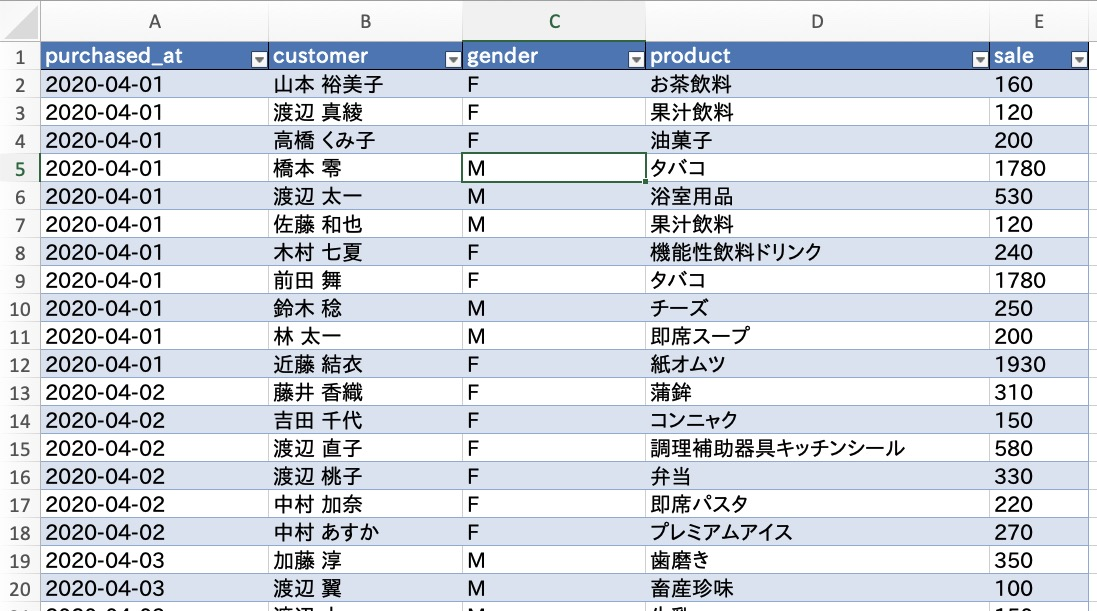
\includegraphics[width=0.9\textwidth]{figure/introduction/yamabata-san-table.jpg}
    \caption{山畑さんが分析に用いた初期のExcelデータの一部．}
    \label{fig:yamabata-san-table}
\end{figure}

図\ref{fig:yamabata-san-table}は，山畑さんが分析の練習材料として用いたExcelデータの一部です．
図を見るとわかるように，このExcelシートでは以下の5項目についてデータが記録されています．
\begin{itemize}
\item \graybox{purchased\_at}: 購買（販売）日時
\item \graybox{customer}: 商品を購入した人物の氏名
\item \graybox{gender}: 商品を購入した人物の性別
\item \graybox{product}: 購入された商品名
\item \graybox{sale}: 販売価格
\end{itemize}

ご存じの通り，Excelはビジネス現場で非常によく使われている表計算ソフトです．
そのすべてを理解している人は少ないですが，データの絞り込みや集計など，便利な機能がたくさん備わっています．
ここでは，山畑さんになりきって以下のクイズに取り組んでみてください．
どのクイズも，販売履歴データの分析においてはよくあるタスクです．


\subsubsection{Q1-購買頻度：あの人は何回買い物をしている？}
Excelの検索機能を用いて，「岡田 真綾」という人物が何回買い物をしていたかを数えてください．

\subsubsection{Q2-購入者の絞り込み：商品Xを購入しているのは誰？}
Excelのオートフィルタ機能を用いて，「ビタミン補助剤」を購入している人をリストアップしてください．

\subsubsection{Q3-総売上金額}
Excel関数の\graybox{\texttt{SUM}}を用いて，現時点での総売上金額を計算してください．

\subsubsection{Q4-人気商品：最も売れた商品は？}
Excelの「ピボットテーブル」機能を使って，集計期間中に
\begin{itemize}
\item 最も購買回数が多かった商品
\item 最も売上金額の合計が大きかった商品
\end{itemize}
をそれぞれ求めてください．

\vspace{2zw}
いかがでしたでしょうか．
Excelの基本的な機能を使えば，どのクイズもサクっと解けたのではないでしょうか．

Excelはビジネス上計算に必要な機能が一通り備わっています．
なにより，大抵のPCにはインストールされているオフィスツールですから，手軽に使えるのが魅力です．
学術研究の世界でも，データの簡単な集計や可視化にはしばしばExcelが使われます．

何も問題がないように見えるExcelですが，扱うデータの規模や用途が大きくなると，様々な問題に遭遇します．
山畑さんのその後の話を例に，その問題点を一緒に考えてみましょう．


% ---------------------------------------
\section{ケース2: サイトの認知度向上につき，得られるデータも膨大に!?}
% ---------------------------------------
現時点では手持ちのデータは少ないものの，販売履歴データの分析に将来性を感じた山畑さん．
販売履歴データを有効活用できるよう，ショッピングサイト運営により力を入れる決意を固めたのでした．

以下は，山畑さんのその後の話（架空の話）です

\begin{framed}
ショッピングサイト立ち上げ以降，順調に利用者数も増えていった．
やはりメディアに取り上げられたのが大きかったのだろう．
あのタイミングでサイトの認知度が一気に高まり，サイトの利用者数や利用頻度も加速度的に増えていった．
それに伴い，サイト運営に関わるスタッフも増員した．

販売履歴の管理は，当初は山畑さんが一人で担当していたが，さすがに一人では対応しきれなくなった．
そこで，ある時点から数名体制で販売履歴の記録を行うことになった．
これまで販売履歴の管理に使ってきたExcelシートをクラウドストレージに置き，記録担当スタッフのPC間で同期を取る仕組みを導入．
同じExcelファイルの上で，スタッフ全員で販売履歴を記録できるようにしたのである．

2年後．サイト事業は軌道に乗った．
十分な量の販売履歴データが蓄積されたと判断した山畑さんは，いよいよ大規模な販売履歴データの分析に取りかかることを決意した．
立ち上げ当初は200〜300行しかなかったExcelシートであったが，シートを開きその行数を数えてみると・・・
なんとその数90万行以上！
データの量に小躍りした山畑さんは，Excelシートの扱いに詳しいスタッフと共に，意気揚々とデータ分析に取りかかったのであった．
\end{framed}

オンラインショッピング事業に成功した山畑さん，蓄積された販売データも膨大な量になりましたね．
90万行以上もあるExcelシートは，まさに「巨大なデータのかたまり」になっています．

さあ，ここからは再度，山畑さんになりきってこのExcelシートを用いたデータ分析に取り組んでみましょう．
こちらのURL（\url{https://github.com/trycycle/database-textbook/raw/refs/heads/main/dataset/purchase\_large.xlsx}）には，上記ケース2で山畑さんが分析しようとしているExcelファイルがあります\footnote{繰り返しになりますが，データはすべて架空のものです．}．
まずは，そのExcelファイル（\graybox{purchase\_large.xlsx}）をダウンロードし，ファイルを開いてください．
このExcelファイルのシートは，先ほどのケース1で用いたExcelシートと同じ構造（項目）となっています．
異なるのは，データの量（行数）だけです．
もし，ファイルがうまく開けない場合は，こちらのURL（\url{https://github.com/trycycle/database-textbook/raw/refs/heads/main/dataset/purchase\_medium.xlsx}）からダウンロードできるExcelファイル（\graybox{purchase\_medium.xlsx}）を用いてください．
ダウンロードが完了したら，ケース1と同じタスク（Q1〜Q4）に取り組んでみてください．
同じタスクでもデータが増えたことで異なる結果が得られるでしょうし，別の体験が得られるはずです．


% ---------------------------------------
\section{表計算ソフトでデータ管理を行ったときに起きる悲劇}
% ---------------------------------------
ケース1および2で用いたExcelファイルは，販売履歴データの集まりでした．
一般的には，このようなデータの集まりは「データベース」ということになるでしょう．

ところで，ケース2のタスクに取り組んでみて，イライラを感じたりしませんでしたか．
実はケース2のExcelファイルには，大量のデータを管理・処理する上での課題を感じていただくために，いくつかの問題を仕込んでおきました．

ファイルを開いた方がまず感じたのは，Excelの動作が重い，ということでしょうか．
Excelは，基本的にデータをすべてメモリに読み込もうとします．
PCのメモリは作業用机のようなものです．
メモリという机が広いほどたくさんの資料（データ）を開いて作業ができますが，机の広さを超えるデータ量を扱おうとすると，PCは身動きが取れなくなってしまいます．
ケース2で扱ったExcelシートは一般的な利用では扱わない量のデータが含まれているため，スペック（メモリ）がそれほど高くないPCを使っている場合，Q1からQ4のタスクに取り組むどころか，Excelファイルを開くことも難しいかもしれません．

無事Excelファイルを開くことができたとしても，ケース2のExcelファイルのデータを分析するには骨が折れます．
まずケース1に比べ，行数が圧倒的に多いです．
そのため，Q1タスクでは，Excelの検索機能を使って「岡田 真綾」さんの行を検索するにしても，データが多すぎて何度も「Enterキー」を押す羽目になります（しかも何回押したか分からなくなる）．
また，ケース2のExcelデータにはデータの誤記や不適切なフォーマットが混入しています．
たとえば，\graybox{sale}の列に半角数字と全角数字が混在しています\footnote{一般に，計算機は半角文字（例: 123，ABC）と全角文字（例: １２３，ＡＢＣ）を区別します．}．
\graybox{purchased\_at}列の日付は，「年\/月\/日」というフォーマットのデータもあれば，「年-月-日」というフォーマットのデータが混在しています．
そのため，Q3タスクでは，売り上げ金額の正しい合計値が得られません（\graybox{SUM}関数は全角数字を無視する）．
さらに，\graybox{product}列では「セル（マス目）1つにつき商品1つ」となっておらず，ある顧客が同時に複数の商品を購入した場合，1つのセルにカンマ区切りで複数の商品が登録されてしまっています．
そのため，Q4タスクではピボットテーブルを使っても，商品ごとの集計が行えなくなっています．

なぜ，このような問題が起きたのでしょうか．
それは，本来Excelは個人用の表計算アプリケーションであって，大規模データの管理や処理を前提として設計されていないためです．
ビジネスの現場で扱うデータは，個人で扱うそれと比べて規模が大きく，多様になることが多いです．
また，複数人，複数部署，複数サービスでデータを共有することも珍しくありません．
そのため，誰かが編集中のデータを別の人が意図せず上書きをしようとしたり，データのフォーマット（形式）や事前に定めた入力ルールを無視してデータを入力してしまう，といった問題も起きやすくなります．
このように，数十万行，数百万行ある表データをExcelで管理・処理しようとすると，さまざまな不都合が生じます（図\ref{fig:excel-disaster}）\footnote{数十万，数百万行の表データはExcelで扱うには大規模ですが，本書で学ぶデータベースシステムにとっては小規模です．現代のデータベースでは，何千万，何億行という規模の表データを扱うことは珍しくありません．}．



\begin{figure}[h]
    \centering
    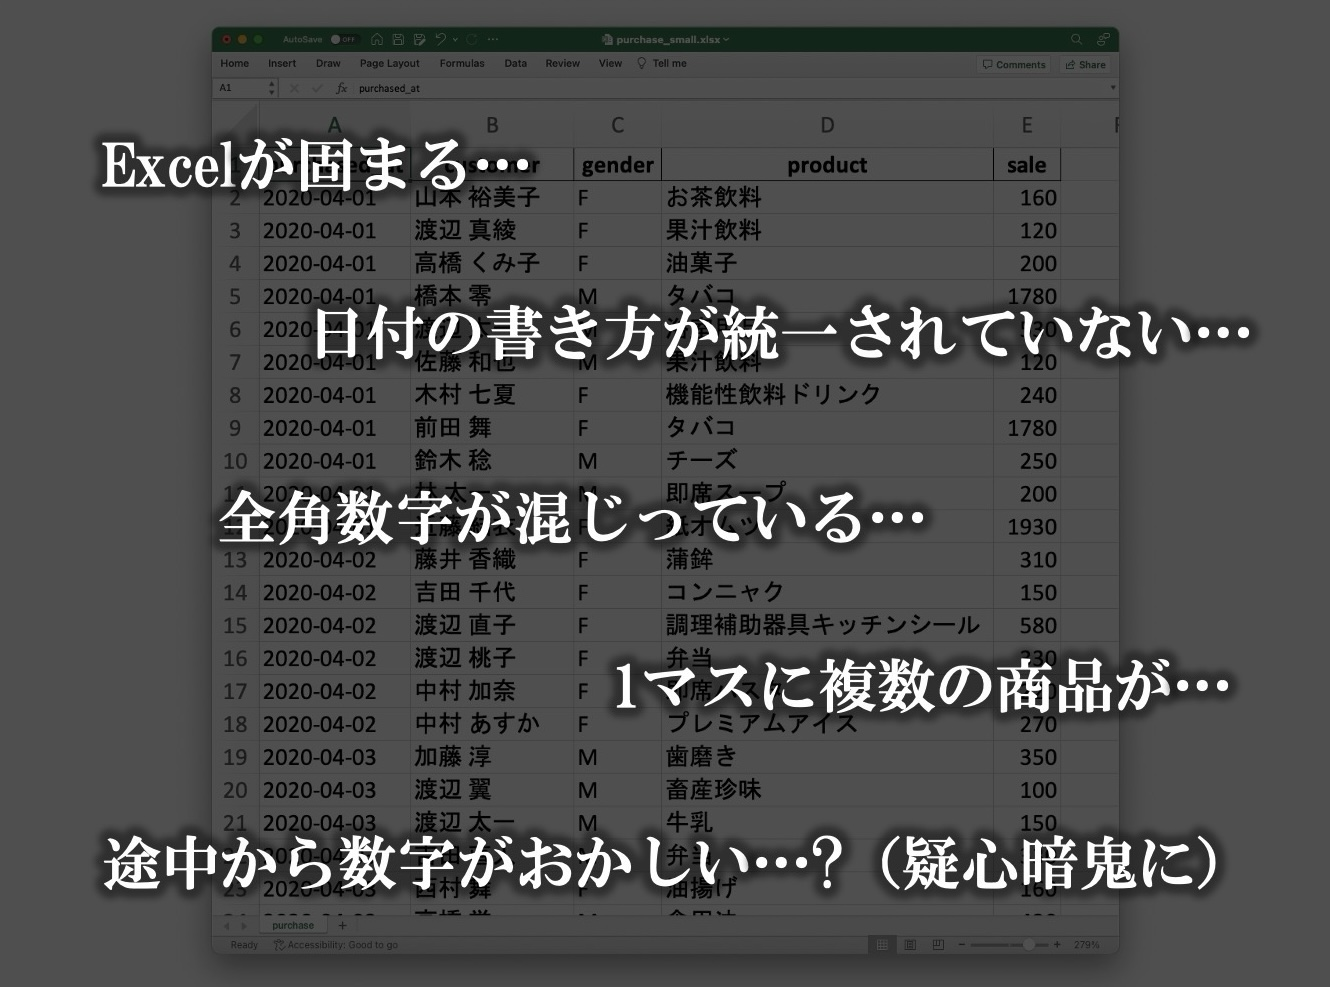
\includegraphics[width=0.8\textwidth]{figure/introduction/excel-disaster.jpg}
    \caption{大きな表データを複数人でExcelで扱うときの悲劇．}
    \label{fig:excel-disaster}
\end{figure}

今日，企業や組織が扱うデータの量はますます増加しています．
また，蓄積された大規模なデータを分析して，ビジネスに活かそうとする動きも活発化しています．
では，大規模なデータをうまく管理・処理するためにはどうすればよいでしょうか．
そのための技術こそが「データベース」です．
「データベース」を用いれば，不適切なデータが混入することを防いだり，大量のデータを効率よく検索・集計することが可能になります\cite{Astrahan1976}．
以降，本書では\strong{大規模データを効率よく管理・処理するための「データベース」技術} について解説します．

